\begin{fullwidth}
\chapter{\label{ch:super_methods}
The syllables superposition experiment}
\end{fullwidth}

\begin{chabstract}

In this chapter we present methods

\end{chabstract}

\section{Methods}

{\label{488128}}

\subsection{Simulation framework}\label{simulation-framework}

We assume that the NBA lives in the cortex, and seek a good compromise between realistic modelling of the cortical dynamics and the tractability of the simulation.
State-of-the-art simulations of larger cortical structures are based on point model neurons that allow the inclusion of biological details such as synaptic dynamics and adaptation, but are restricted to about the size of a cortical column \cite{potjans2012cell}.
For larger scale networks, such as ours, a population-based approach is currently the only feasible approach.
The two choices are: rate based models or population density techniques (PDTs).
In rate based models, the population is described by a single variable, usually related to the population firing rate or average membrane potential of neurons in the population. 
A prominent example is the  Wilson-Cowan equation \cite{wilson1972excitatory}, which describes the dynamics of the population activity as a first order linear differential equation driven by inputs.
Another example is the Jansen-Rit model \cite{jansen1995electroencephalogram}, which is primarily motivated by phenomenological considerations.
In both examples, the relationship with the underlying neural state is unclear. We have opted for PDTs, also a population based approach, but one where the relationship with the dynamics of a group of spiking point model neurons can be made rigorous.
Although they are computationally more expensive than rate based models, they are easier to manage than a full-blown model using spiking neurons, which would need hundreds of thousands of neurons at the scale of the cortical network considered here.
We will briefly set out the assumptions that we use in modelling populations and describe the numerical methods involved.

Consider a leaky-integrate-and-fire (LIF) neuron, which is characterized by a single state variable: the membrane potential.
If the neuron has a potential different from its equilibrium potential, or when it experiences an external drive, for example generated by a synaptic current, the potential evolves according to:

\begin{equation}
\tau \frac{dV}{dt} = -(V - V_{rev}) + I(t).
\label{eq-lif}
\end{equation}

Here $V$ is the membrane potential in V, $\tau$ the membrane time constant in s, $V_{rev}$ the reversal potential and $I(t)$ and external current, which may comprise contributions from other neurons in the form of spikes, and therefore may be stochastic.
If the membrane is driven far above the equilibrium potential, at a potential $V_{th}$, the threshold, the neuron spikes.
We assume it will be inactive for an absolute refractive period $\tau_{ref}$ and then finds itself reset to the equilibrium potential after that.  
This scenario is easy to simulate: using a simulator like NEST \cite{gewaltig2007nest}, or BRIAN \cite{stimberg2014equation}, one can create populations of LIF neurons.
In the simplest case a population is driven by synthetically generated input spike trains, where the spike train events are created by a random generators.
The default assumption is that inter-spike intervals are Poisson distributed, although this can be extended to non-Markov processes \cite{lai2017population}.
It is clear that $I(t)$ in Eq. \ref{eq-lif} now should be considered as a stochastic variable and that the threshold crossings of LIF neurons themselves are stochastic events as a consequence.
Fig. \ref{fig:pdt-case} A  demonstrates a simple scenario: a population of 10000 LIF neurons, driven by a stochastic input - Poisson generated spike trains, where each LIF neuron experiences about 800 input spikes per second.
The simulation shows a spike raster of the population response:
first nothing: although each LIF neuron receives input spikes and as a consequence has its membrane potential driven up, none of the neurons have reached threshold;
then a spike volley: most neurons hit threshold at approximately the same time;
followed by a period of relative silence: only interrupted by a few stragglers;
at last a gradually achieved final neural state of asynchronous random firing.
More complex networks can be formed by feeding the output spikes of one population into other populations.

This is a fascinating but unwieldy process and statistical methods have been used to describe it at the population level \cite{stein1967some,knight1972dynamics,omurtag2000simulation}.
A population is described by a density function, which expresses how the population is distributed over state space.
For LIF neurons this is a function $\rho(V)$, where $\rho(V)dV$ is the fraction of neurons with their membrane potential in interval $[V, V + dV)$ (when we integrate the density function over a certain state interval, we will refer to the  result as  the amount of \emph{mass} in that interval).
The initial distribution of the neurons in the population must be chosen, but the evolution of the density is tractable.
It is clear that neurons move through state space due to the deterministic neural dynamics, Eq \ref{eq-lif} for LIF neurons, and also go transitions due to the input spikes.
The collective contribution of the stochastic process to the evolution of the density profile can be  modelled using a Poisson master equation \cite{crispin1994handbook}; the contribution of the deterministic dynamics  can be modelled using an advection equation (see \cite{omurtag2000simulation} for a lucid explanation). 


As a consequence, the process of simulating thousands of neurons is now replaced by modelling the evolution of a density which is given by a single equation:

\begin{equation}
\frac{\partial \rho}{\partial t} -\frac{1}{\tau}\frac{\partial}{\partial v}(\rho v) = \int dh p(h) \nu (\rho(v - h) -\rho(v)),
\label{eq-synapse}
\end{equation} 

Here $p(h)$ is the distribution of synaptic efficacies, $\nu$ the frequency of the incoming spike trains, $\rho$ the density function, $t$ the time since start of simulation and $v$ the membrane potential.
Mass that is being pushed across threshold corresponds to neurons spiking; consequently  the firing rate of the population can be calculated directly from the mass flux across threshold.

Efficient and stable simulation methods are available \cite{nykamp2000population, de2003simple, de2013generic, iyer2013influence}, and remarkably, the process of solving Eq. \ref{eq-synapse} is computationally less expensive for LIF neurons than the direct simulation using NEST \cite{nykamp2000population}.
The process of keeping track of a single density function, and the communication between populations using firing rates rather than individual spikes, frees the modeller from keeping track of thousands of spikes per second and leads to simpler simulations.
Figure \ref{fig:pdt-case} shows the very close correspondence between direct simulations of LIF spiking neurons and population density results.
It shows, first, that the simulation results indeed are very close to that of the spiking simulation, and second, that Wilson-Cowan dynamics must be tuned in a way that PDTs do not: the correct steady state activation must be provided to the Wilson-Cowan dynamics in the form of a sigmoid, while in PDTs the correct steady state firing rate is calculated from first principles - input firing rate, synaptic efficacies and neural parameters - without any need for tuning. 


\begin{figure}[h!]
  \begin{center}
    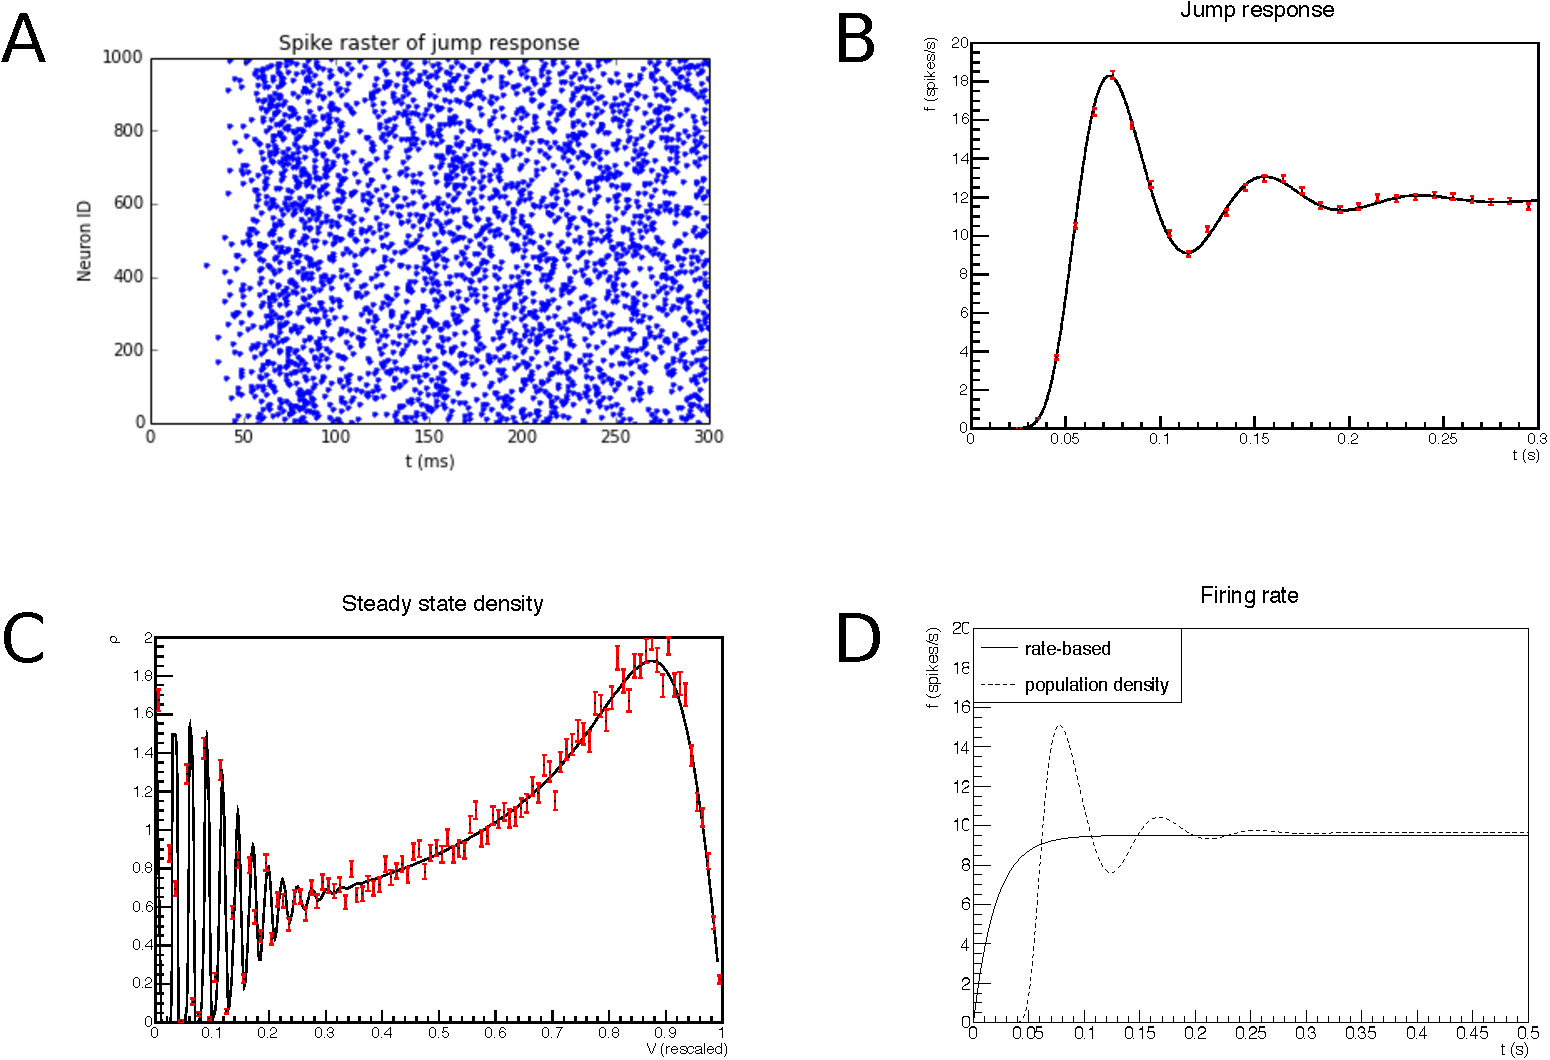
\includegraphics[width=1.0\columnwidth]{figures/pdt_overview.pdf}

    \caption{\textbf{A.} A spike raster showing an LIF population undergoing a jump response.
        Neurons are at equilbrium at $t = 0$. From $t=0$ each neuron receives a Poisson distributed input spike train ($\lambda$ = 800 Hz, $h= 0.03$, i.e. an input spike raises the PSP by 3\% of the difference between threshold and equilibrium potential, $\tau = 50$ ms, following \cite{omurtag2000simulation}).
        \textbf{B.} Firing rate calculated from the PDT method (solid curve), compared to firing rate from spiking neuron simulation (red markers).
        \textbf{C.} The density calculated by the PDT method (solid curve) at $t=0.3$ s, compared to a histogram of the membrane potential over the population at the
        same time.
        \textbf{D.} Wilson-Cowan prediction for the firing rate, compared to PDT result. Importantly, Wilson-Cowan output must be tuned: the steady state value to which it converges is not predicted by the Wilson-Cowan equations, but must be provided as a sigmoid. 
       In contrast, the PDT method calculates the firing rate from first priciples, and agrees well with the spiking neuron simulation, within statistics.
      }
\label{fig:pdt-case}
  \end{center}
\end{figure}


The population density formalism can be extended to higher dimensional models.
For example, the adaptive-exponential-integrate-and-fire neuron (AdEx) \cite{brette2005adaptive} is a two dimensional model that has the membrane potential and an adaptivity parameter as a variable.
Consequently, the state space is two dimensional.
The motivation behind this model is that first, it includes adaptation, and second that it is the effective approximation of the complex conductance-based processes that take place in a real neuron.
The equations of the model are:

We consider the AdEx model as presented by Brette and Gerstner \cite{brette2005adaptive}, which describes individual neurons by the following equations:
\begin{align}
  C_m \frac{dV}{dt}    & =  -g_l(V - E_l)  + g_l e^{ \frac{(V - V_T)}{\Delta_{T}}} \\
  \tau_w \frac{dw}{dt} & =  a(V-E_l) -w \nonumber
\end{align}

Where $C_m$ is the membrane capacitance, $g_l$ the leak conductance, $E_l$ the leak potential (equivalent to the reversal potential for the LIF), $V_T$ a threshold potential, $\Delta_T$ a shape parameter for the spike, $\tau_w$ the adaptation time constant, $a$ the subthreshold adaptation parameter,  $V$ the membrane potential and $w$ the adaptation parameter. Upon a spike, the neuron is undergoes a transition in $w$: $w \rightarrow w +b$, where $b$ is the spike adaptation parameter.
We use the parameters given by Brette and Gerstner (2005).


\begin{figure}[h!]
  \begin{center}
    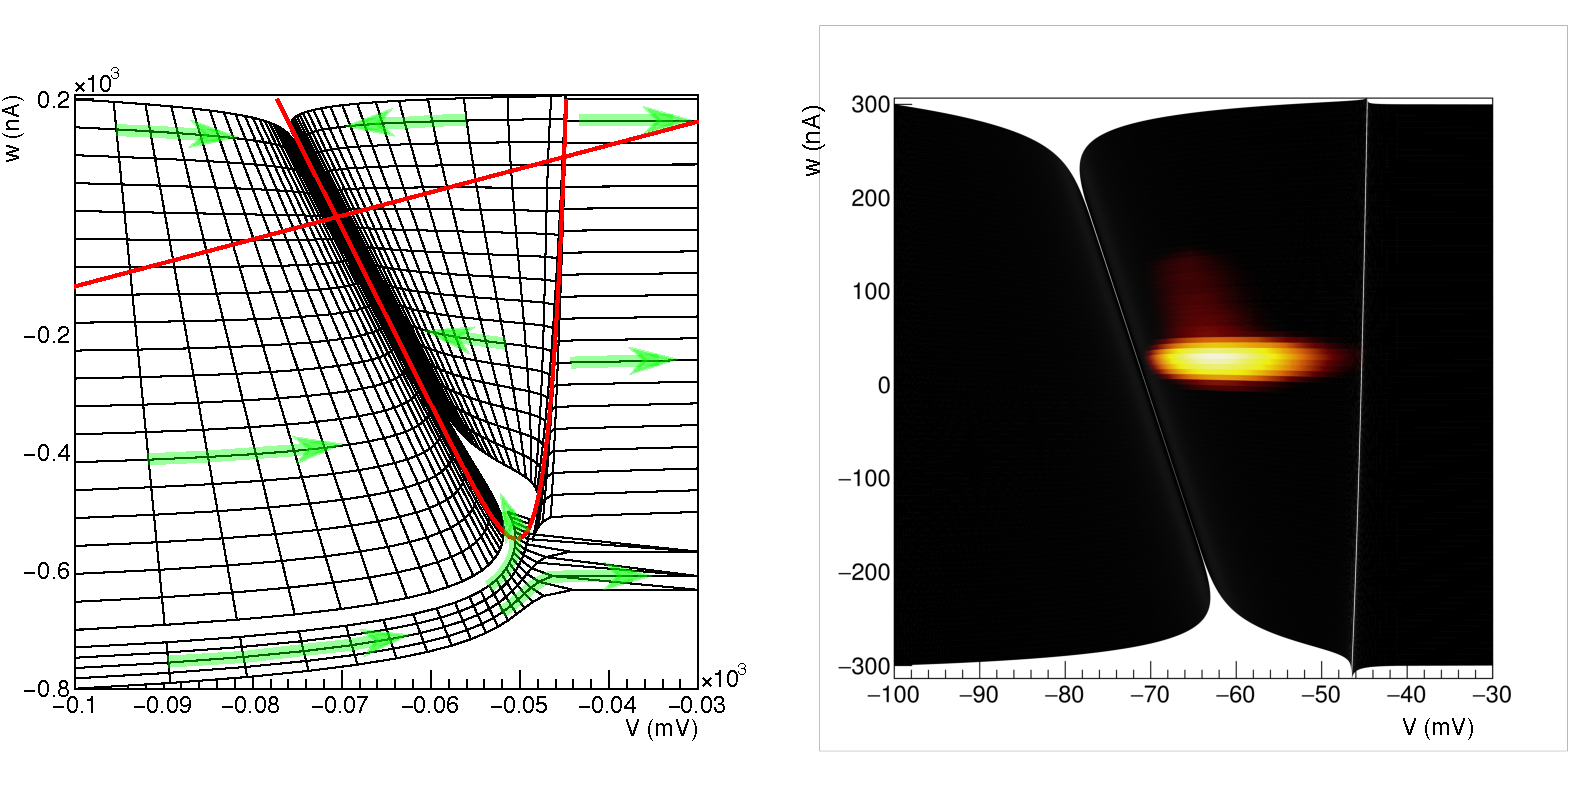
\includegraphics[width=1.0\columnwidth]{figures/aexp_overview.pdf}
    \caption{{AdEx dynamics {\label{fig-adex}} Left: Overview of AdEx dynamics.
        Right: a heat plot of the density profile during simulation. On the horizontal axis the membrane potential, on the vertical axis the adaptivity parameter. Note that
 the right figure constitutes a considerable reduction of state space compared to left. For the connectivity parameters we use, the state space on the right is the
part of state space reachable by dynamics.
      }}
  \end{center}
\end{figure}

We illustrate the dynamics of the neuron in Fig. \ref{fig-adex}.
The direction of the dynamics is shown by arrows, the speed of the dynamics by the size of the cells:
big cells implies fast dynamics as the cells represent equidistant time steps.
This shows that at $w =0$ dynamics are leaky,  i.e. towards the equilibrium, except at high values of $V$, on the right, which corresponds to spike generation.
At high values of $w$, there are two effects: stronger leak (larger cells) and a lower (more negative) equilibrium potential, which makes it harder for a cell at high $w$ to be driven across threshold, precisely the effect one expects due to adaptation.
At low $w$, the opposite happens: cells become more excitable.
For very low $w$ values, which can not be reached under cortical conditions, at least not for the parameters we used, there is the theoretical probability of a rebound (neuron always spikes).

A density function now lives in this two dimensional space: $\rho(V,w)$.
The evolution equation is a direct generalization of Eq. \ref{eq-synapse}.
For a model with $n$ state variables $\vec{V}$, a point model takes the form:
\begin{equation}
\tau \frac{d \vec{V}}{dt} = \vec{F}(\vec{V})
\end{equation}
and the density equation:
\begin{equation}
\frac{\partial \rho}{\partial t} + \frac{\partial}{\partial \vec{V}} \cdot \frac{( \vec{F} \rho)}{\tau} = \int dh p(h) \nu (\rho(\vec{V} - \vec{h}) -\rho(\vec{V}))
\end{equation},
where $\vec{h}$ represents the effect of an input spike.

We represent the density function by a heat plot on state space: the highest values or white, low values are red.
We are able to simulate the density function by a method analogous to that of \cite{de2013generica,iyer2013influence}, generalized to two dimensions.
In Fig. \ref{fig-adex} we show the result of a simulation: the density function as a fixed point in time.
As before, we can calculate the firing rate of the population by calculating the the flux across threshold (which is still given by $V= V_{threshold}$, i.e. the right hand side of the grid).

The simulation software, MIIND, is publicly available \url{http://miind.sf.net}. The LIF version of the algorithm has been available for some time \cite{de_Kamps_2008}, while 
the two dimensional version has become available recently \cite{dekamps2017b}.


\subsection{NBA simulation}\label{architectural-decisions}

Previous simulations of the NBA approximate the mean activity of neural assemblies with Wilson Cowan dynamics \cite{Frank_2014}.
Nonetheless, as explained in section \ref{simulation-framework}, direct simulations of leaky-integrate-and-fire (LIF) neurons \cite{omurtag2000simulation} have different transient behaviour than the dynamics described by the Wilson Cowan equations.Since we are interested in modelling the transient dynamics of variable binding in order to compare 
the simulation with real temporally detailed patterns of intracortical neural measurements like ECoG, we feel the need to model spiking neuron dynamics is important.

The decision to use AdEx, rather than LIF neurons has two motivations: first, adaptation is ubiquitous and its inclusion has a substantial impact on the dynamical range
allowed within the constraints of the blackboard architecture. Second,  it has been shown that 2D models, like AdEx, can already predict correctly 96\% of the spikes of 
detailed conductance models\cite{brette2005adaptive}.  Also, this model reproduces many known electrophysiological features, as can be appreciated in the spike-frequency adaptation review of Benda et al. \cite{Benda_2003,Benda_2014}. Our approach is consistent with a trend towards simpler, geometrically motivated  2D   models  that preserve the essence of more complex biophysically motivated models \cite{izhikevich2007dynamical}.

AdEx is now available in  MIIND. To our knowledge this is the first time that the AdEx model will be employed to approximate the neural dynamics of a circuit of this magnitude reproducing cognitive function.

In the case of Delay Activity (DA) populations like Working Memory (WM), we decided as a first approach to model such a mechanism phenomenologically.
We plan to address the different alternatives to model persistent cortical activity with interacting neural populations in future work.
As suggested by de Kamps\cite{de_Kamps_2005} not only models of recurrent excitation but also recurrent inhibition can account for this phenomena.
In the current simulation, a constant firing rate for DAs is kicked off by a specified level of input, resulting in activation  that is sustained for a predetermined period of time.
Contrary to previous simulations \cite{velde2015ambiguity}, we do not consider Sub-Assemblies (SAs) as DA populations.
We find that SAs can show rich and interesting dynamics just by fulfilling their function of mediating activation for WM.

We model Main-Assemblies (MAs)  as receiving input from DA populations, representing word types in some cases, and WM populations representing phrase types in other cases.
We do this to satisfy the assumptions of a phrase grammar that requires representation of deep tree hierarchical structures, so that we can separate the notion of a phrase resulting from previous word type bindings stored in WM, from the recruitment of MAs representing word grammatical category instantiations that take place during sentence processing.
Note that for other grammar types, like dependency grammars considered in previous NBA simulations\cite{velde2015ambiguity}, to consider words as nodes in their syntactic representations, we would only need to model word types for the MAs of the necessary compartment circuits.


\subsection{Compartment circuit parameters}\label{sec:circuit-parameters}

The compartment circuit contains two different types of neural populations.
Artificial neural populations following a boxcar event model, shown in Figure \ref{fig:circuit-spec}.B and biological neural populations following LIF or AdEx neural models.
We took LIF parameters from Omurtag et al. (2000) \cite{omurtag2000simulation} and AdEx parameters
from Brette and Gertsner \cite{Brette_2005}.

\begin{figure}[h!]
  \begin{center}
    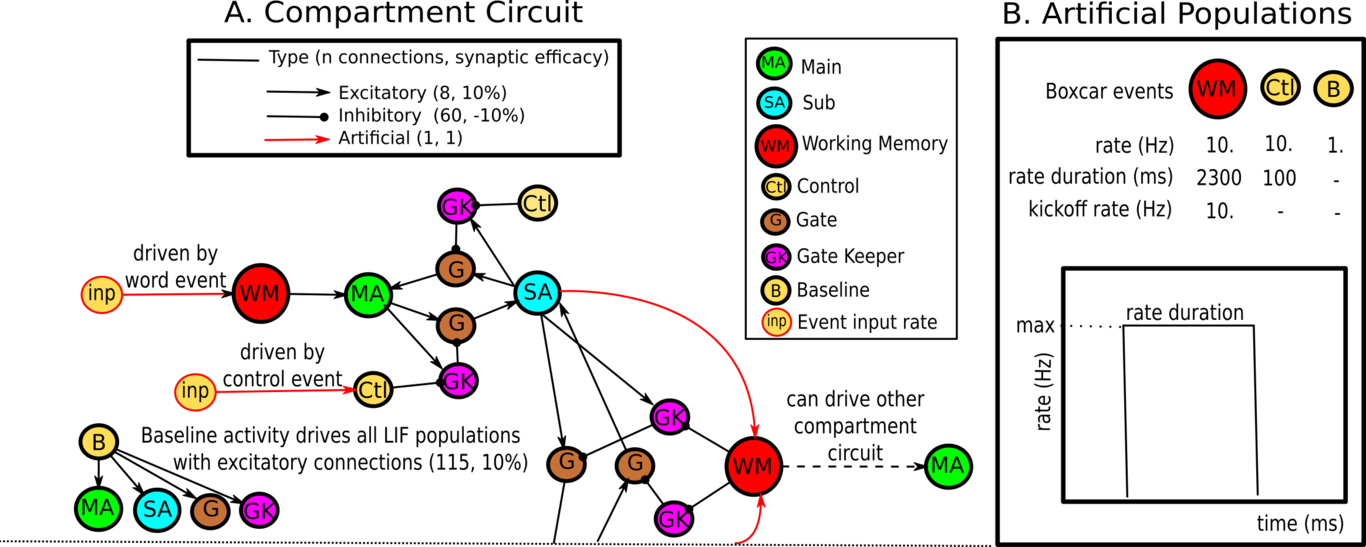
\includegraphics[width=1.00\columnwidth]{figures/circuit_specs3}
    \caption{{Compartment circuit example {\label{fig:circuit-spec}} A.
Details
        of the Compartment Circuit implementation.
Only half of the
        circuit is shown since the design is symmetric.
The baseline
        (B) and Event input (Inp) populations are part of the
        simulation and not of the original abstract circuit proposal.
        B.
The behavior of the artificial neural populations and their
        selected parameters is shown%
      }}
  \end{center}
\end{figure}

As a first step we wanted to only explore the general behavior of the circuit of neural populations following well studied sets of parameters.
Nonetheless it is clear that studying the neural dynamics of specific brain regions might require adapting the parameters of the neural models to local measurements.
Each neural population is either excitatory or inhibitory; this means that a population that is excitatory (inhibitory) on one population is excitatory (inhibitory) on others as well, respecting Dale's law.

The dynamics of most populations are given by the PDTs and ultimately determined by the underlying model of spiking neurons.
These neural populations comprise a pair of Main Assemblies (MA), a pair of Sub Assemblies (SA), six Gate Assemblies (G) and six Gate Keeper Assemblies (GK).

Nonetheless there are a few other populations for which we simplified the simulation to the phenomenological level with an imitation of Delay Activity, which means that, after transient stimulation, a population retains its activation above a certain threshold for a given period of time.
For instance, the biophysical mechanisms of WM are still not understood completely, but its characterization as Delay Activity is relatively uncontroversial.
We modelled in this way, Control assemblies (Ctl), Working memory assemblies (WM), Event Input Assemblies (Inp) and a Baseline Assembly (B) that drives baseline neural activity of all completely simulated neural populations.
A complete diagram of the compartment circuit with example parameter values for LIF populations is given in Figure \ref{fig:circuit-spec}.\\~\\

We use a boxcar event model for persistent activity.
This model requires specification of the starting point of events, the persistent firing rate of the population and the duration of the persistent activity.
In the case of the Delay Activity of WM we also have to provide a kickoff input rate threshold that automatically triggers the boxcar event instead of providing a start time point.
The duration of persistent activity was pragmatically set up long enough for the neural dynamics to reach steady state and allow the formation of  all required bindings between phrase types and 
word types.
Finally the persistent activity rate and kickoff rate threshold were arbitrarily selected from possible parameter range values as a result of simulations of the circuit dynamics that will become clear in the following section.

Selecting firing rates to tune the compartment circuit is a complex task given the contrast between the extremely simplified circuit and real neural networks that contain multiple types of neurons with diverging behavior across cortical layers \cite{Wohrer_2013}.
Wohrer et al \cite{Wohrer_2013} show, from measurements in rat cortex, that the actual firing rate distributions of neural networks do not differ much between resting state and evoked activity.
The small difference would come from very few neurons that manage to drive up the mean firing rate in recordings while most neurons in the population are almost silent, some with rates as low as 0.1 Hz \cite{Kerr_2005}, whose activity might not even be picked up by most recording devices.
Although theoretical analysis of the distribution of firing rates in randomly recurrently connected networks of LIF neurons near the fluctuation-driven regime suggests considering mean firing rates around 6.4 Hz \cite{Roxin_2011}.
Based on the review of Wohrer et al. \cite{Wohrer_2013}, particularly on the firing rate in motor areas of behaving macaques, we decided to kickstart biological neural populations activity up to a conservative baseline firing rate of 1 Hz and study the neural dynamics of circuit input firing rates of up to 10Hz.

There are two parameters governing transmission of neural activity between neural populations.
First, the synaptic efficacy of connections, which was setup to be uniform across the circuit under the lack of appropriate hypothesis to tinker it in a detailed manner. According to London \cite{London_2002}, current understanding of synapsis is limited and contextual measurements and parametrization of efficacy might be more appropriate than fixing individual connection parameters.
For example recent evidence \cite{Briggs_2013} shows that synaptic efficacy might be modulated by attention processes.
In the study of Briggs \cite{Briggs_2013} neurons of the thalamus were stimulated while measuring evoked responses from corresponding monosynaptically connected neurons in primary visual cortex.
With this procedure the authors showed that, the percentage of shocks that evoke a postsynaptic response, the average efficacy, ranged from 28\% to 36\% depending on the type of neurons considered and the attention state.
Considering the possible efficacy variability in cortex, we decided to verify, through simulations of a sub-circuit, the sensitivity of the circuit temporal dynamics to low (10\%) and high (30\%) values of synaptic efficacy, where percentages are taken with respect to the difference between equilibrium and threshold potential, for both LIF and AdEx populations.

The second parameter governing transmission of neural activity was the number of connections between a pair of neural populations.
Unlike synaptic efficacy, the number of connections were determined from a series of simulation experiments.
First the number of connections from baseline persistent activity was set such that, during rest, the circuit steady state activity would stabilize around 1 Hz.
The number of baseline connections necessary is a function of input firing rate, synaptic efficacy and neural model, such that a lower synaptic efficacy required a higher number of connections.
Then the number of connections coming from excitatory populations was determined such that bidirectional gating circuits would have a stable steady state firing rate when both Gs allow neural activity to be transmitted.
Finally the number of connections coming from inhibitory nodes were setup high enough to block neural activity flow in a gating circuit, which means that GKs driven by MAs would be able to completely inhibit activity in Gs.
Our simple approach to neural rate transmission ignores many intricacies like activity regimes that might allow rich internal computations.
\cite{Ostojic_2014}.
Also connections distribution might have an impact in spike based communication \cite{Teramae_2012}.
Still we decided to keep connections between populations as simple and homogeneous as possible for a first approach.

\subsection{Simulation experiments performed}\label{simulation-experiments-performed}

Since it is possible to tune the circuit to reproduce a wide range of firing rate absolute values under which circuit dynamics are similar and stable, we simply aimed at picking reasonable parameter values such that the circuit would maintain overall modest firing rate values with respect to the literature of neural measurements.
To setup parameters and compare in detail the compartment circuit dynamics for LIF and AdEx neural populations, four simulation experiments were performed taking different sub-circuits into account.
A diagram of each sub-circuit is shown in Figure \ref{sub_circuits}.

\begin{figure}[h!]
  \begin{center}
    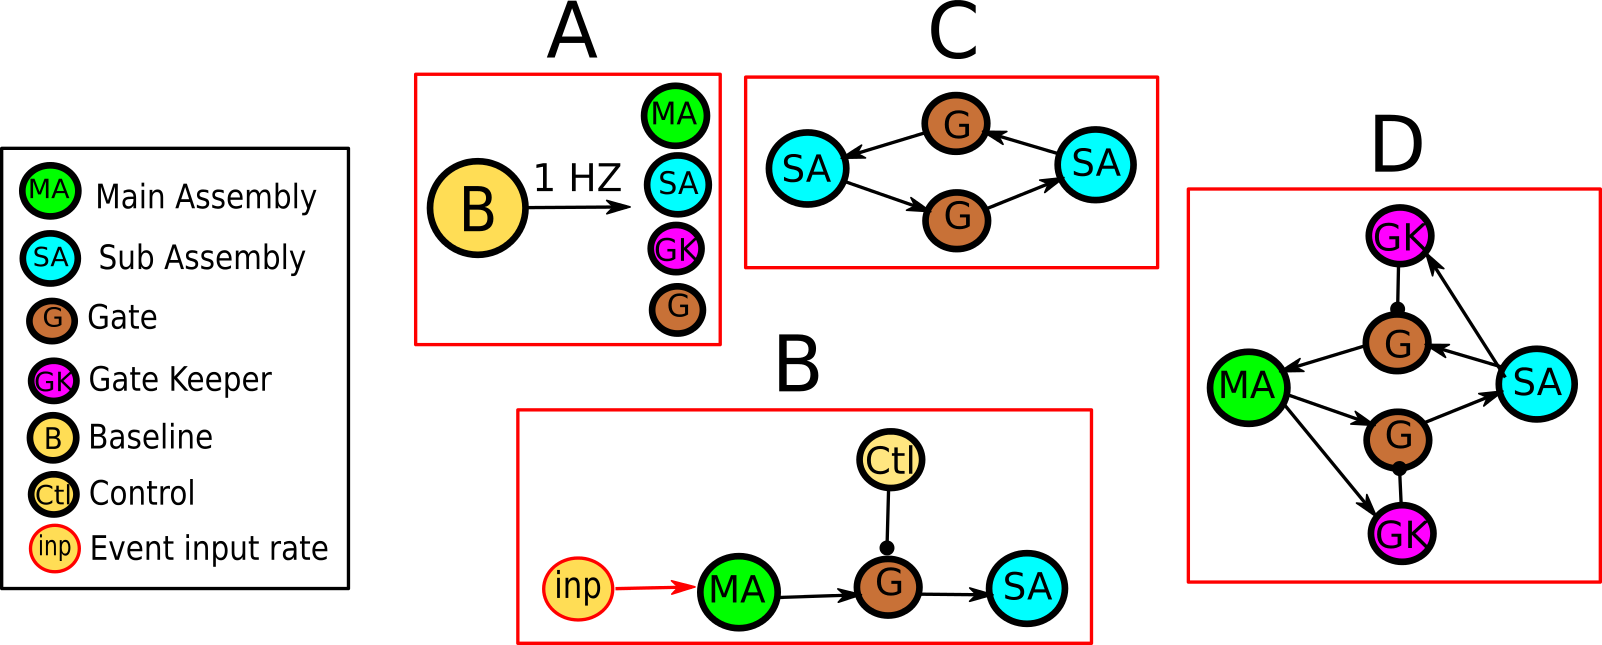
\includegraphics[width=0.9\columnwidth]{figures/sub_circuits}
    \caption{Sub-circuit simulation topologies.
      For better visualization baseline activity nodes are excluded from the topologies.
      A. Single neural population driven by baseline activity.
      This topology~ reminds of the fact that all MA, SA, G and GK populations are driven initially in the same way by a persistent baseline fixed rate.
      B. Chain of populations where activity is temporally interrupted by a control node.
      C. Excitatory loop between SAs when Working Memory is activated.
      D. Excitatory loop broken thanks to GKs inhibition. {\label{sub_circuits}}%
    }
  \end{center}
\end{figure}

The first simulation simply consists of the activity of one neural population driven by a fixed activity rate of 1 Hz.
We used this simulation to explore the necessary number of baseline connections to drive baseline activity in the circuit to approximately 1 Hz.
The second simulation allowed us to explore how neural activity flows through a chain of neural populations being regulated by a control mechanism.
The third simulation explores how neural activity is enhanced by a closed loop between a MA and SA, since it will be the case in the memory sub-circuit that activity is allowed to flow bidirectionally once the WM delay activity is unleashed.
Finally the fourth simulation consists on adding GKs to the closed loop sub-circuit of the second simulation to explore how many inhibitory connections are necessary to keep activity from flowing in the circuit unless the control mechanism allows it.

After determining reasonable parameter values, we simulated the complete circuit, shown in Figure \ref{fig:circuit-spec}, for both LIF and AdEX neural populations.
Then we compared the resulting neural patterns of the MA, SA, G and GK neural populations to binding and constituency effects available in the neuroimaging literature.

We simulated the binding activity related to the processing of complete phrases, by assuming a syntactic tree structure given by a phrase grammar and the order of control events given by a bottom up parsing scheme.
As a first simplified approximation to the NBA dynamics, we instantiated the required compartment circuits independently to represent the complete assumed tree structure and temporally align their neural signals according to input onsets.
Like this we obtained entire phrase neural time series, by summing activity across similar node categories of the multiple independent compartment circuits instantiated.
We used this procedure to simulate the neural activity of simple phrases, corresponding to increasing size right branching tree structures, to be compared with two different neuroimaging signals.

First, we showed similarities between the activity of simple phrases and ECoG time series patterns of binding revealed by Nelson et al\cite{Nelson_2017}. 
We naively compared the firing rates of our simulation directly to the patterns observed in ECoG recordings, considering the correlation that exist between the high gamma power of local field potential signals and firing rates\cite{Ray_2011,Manning_2009}.
Nonetheless a quantitative comparison would require a more careful consideration, employing recent models tuned to electro-physiological measurements that offer a way to translate neural activity to local field potentials\cite{Mazzoni_2015,Hagen_2015}.

Second, we concatenated simple phrases to reproduce the stimuli of Pallier \emph{et al.} (2011)\cite{Pallier_2011}.
Then we convolved the stimuli neural time series with the Glover Hemodynamic Response Function\cite{Glover_1999}.
This allowed us to make a qualitative comparison with the hemodynamic constituency effects depicted by Pallier et al. (2011)\cite{Pallier_2011}.

Since the quantitative level of neural activity can be easily tuned for a wide range of parameter values with similar behavior, when comparing the circuit neural dynamics with the neuroimaging literature, we only focused on the qualitative neural temporal patterns observed.
All the C++ scripts behind the circuit and sub-circuit simulations, taking advantage of the MIIND software\cite{de_Kamps_2008}, are accessible in the Blackboard application folder of the MIIND github repository at https://github.com/dekamps/miind.